
% Note that the a4paper option is mainly intended so that authors in
% countries using A4 can easily print to A4 and see how their papers will
% look in print - the typesetting of the document will not typically be
% affected with changes in paper size (but the bottom and side margins will).
% Use the testflow package mentioned above to verify correct handling of
% both paper sizes by the user's LaTeX system.
%
% Also note that the "draftcls" or "draftclsnofoot", not "draft", option
% should be used if it is desired that the figures are to be displayed in
% draft mode.
%
\documentclass[conference]{IEEEtran}


% *** CITATION PACKAGES ***
%
\usepackage{cite}


% *** GRAPHICS RELATED PACKAGES ***
%
\ifCLASSINFOpdf
  \usepackage[pdftex]{graphicx}
  % declare the path(s) where your graphic files are
  % \graphicspath{{../pdf/}{../jpeg/}}
  % and their extensions so you won't have to specify these with
  % every instance of \includegraphics
  \DeclareGraphicsExtensions{.pdf,.jpeg,.png}
\else
  % or other class option (dvipsone, dvipdf, if not using dvips). graphicx
  % will default to the driver specified in the system graphics.cfg if no
  % driver is specified.
  \usepackage[dvips]{graphicx}
  % declare the path(s) where your graphic files are
  % \graphicspath{{../eps/}}
  % and their extensions so you won't have to specify these with
  % every instance of \includegraphics
  \DeclareGraphicsExtensions{.eps}
\fi

% *** MATH PACKAGES ***
%
%\usepackage[cmex10]{amsmath}
% A popular package from the American Mathematical Society that provides
% many useful and powerful commands for dealing with mathematics. If using
% it, be sure to load this package with the cmex10 option to ensure that
% only type 1 fonts will utilized at all point sizes. Without this option,
% it is possible that some math symbols, particularly those within
% footnotes, will be rendered in bitmap form which will result in a
% document that can not be IEEE Xplore compliant!
%
% Also, note that the amsmath package sets \interdisplaylinepenalty to 10000
% thus preventing page breaks from occurring within multiline equations. Use:
%\interdisplaylinepenalty=2500
% after loading amsmath to restore such page breaks as IEEEtran.cls normally
% does. amsmath.sty is already installed on most LaTeX systems. The latest
% version and documentation can be obtained at:
% http://www.ctan.org/tex-archive/macros/latex/required/amslatex/math/



% *** SPECIALIZED LIST PACKAGES ***
%
%\usepackage{algorithmic}
% algorithmic.sty was written by Peter Williams and Rogerio Brito.
% This package provides an algorithmic environment fo describing algorithms.
% You can use the algorithmic environment in-text or within a figure
% environment to provide for a floating algorithm. Do NOT use the algorithm
% floating environment provided by algorithm.sty (by the same authors) or
% algorithm2e.sty (by Christophe Fiorio) as IEEE does not use dedicated
% algorithm float types and packages that provide these will not provide
% correct IEEE style captions. The latest version and documentation of
% algorithmic.sty can be obtained at:
% http://www.ctan.org/tex-archive/macros/latex/contrib/algorithms/
% There is also a support site at:
% http://algorithms.berlios.de/index.html
% Also of interest may be the (relatively newer and more customizable)
% algorithmicx.sty package by Szasz Janos:
% http://www.ctan.org/tex-archive/macros/latex/contrib/algorithmicx/


% *** ALIGNMENT PACKAGES ***
%
%\usepackage{array}
% Frank Mittelbach's and David Carlisle's array.sty patches and improves
% the standard LaTeX2e array and tabular environments to provide better
% appearance and additional user controls. As the default LaTeX2e table
% generation code is lacking to the point of almost being broken with
% respect to the quality of the end results, all users are strongly
% advised to use an enhanced (at the very least that provided by array.sty)
% set of table tools. array.sty is already installed on most systems. The
% latest version and documentation can be obtained at:
% http://www.ctan.org/tex-archive/macros/latex/required/tools/


%\usepackage{mdwmath}
%\usepackage{mdwtab}
% Also highly recommended is Mark Wooding's extremely powerful MDW tools,
% especially mdwmath.sty and mdwtab.sty which are used to format equations
% and tables, respectively. The MDWtools set is already installed on most
% LaTeX systems. The lastest version and documentation is available at:
% http://www.ctan.org/tex-archive/macros/latex/contrib/mdwtools/


% IEEEtran contains the IEEEeqnarray family of commands that can be used to
% generate multiline equations as well as matrices, tables, etc., of high
% quality.


%\usepackage{eqparbox}
% Also of notable interest is Scott Pakin's eqparbox package for creating
% (automatically sized) equal width boxes - aka "natural width parboxes".
% Available at:
% http://www.ctan.org/tex-archive/macros/latex/contrib/eqparbox/


% *** SUBFIGURE PACKAGES ***
%\usepackage[tight,footnotesize]{subfigure}
% subfigure.sty was written by Steven Douglas Cochran. This package makes it
% easy to put subfigures in your figures. e.g., "Figure 1a and 1b". For IEEE
% work, it is a good idea to load it with the tight package option to reduce
% the amount of white space around the subfigures. subfigure.sty is already
% installed on most LaTeX systems. The latest version and documentation can
% be obtained at:
% http://www.ctan.org/tex-archive/obsolete/macros/latex/contrib/subfigure/
% subfigure.sty has been superceeded by subfig.sty.


%\usepackage[caption=false]{caption}
%\usepackage[font=footnotesize]{subfig}
% subfig.sty, also written by Steven Douglas Cochran, is the modern
% replacement for subfigure.sty. However, subfig.sty requires and
% automatically loads Axel Sommerfeldt's caption.sty which will override
% IEEEtran.cls handling of captions and this will result in nonIEEE style
% figure/table captions. To prevent this problem, be sure and preload
% caption.sty with its "caption=false" package option. This is will preserve
% IEEEtran.cls handing of captions. Version 1.3 (2005/06/28) and later 
% (recommended due to many improvements over 1.2) of subfig.sty supports
% the caption=false option directly:
\usepackage[caption=false,font=footnotesize]{subfig}
%
% The latest version and documentation can be obtained at:
% http://www.ctan.org/tex-archive/macros/latex/contrib/subfig/
% The latest version and documentation of caption.sty can be obtained at:
% http://www.ctan.org/tex-archive/macros/latex/contrib/caption/


% *** FLOAT PACKAGES ***
%
%\usepackage{fixltx2e}
% fixltx2e, the successor to the earlier fix2col.sty, was written by
% Frank Mittelbach and David Carlisle. This package corrects a few problems
% in the LaTeX2e kernel, the most notable of which is that in current
% LaTeX2e releases, the ordering of single and double column floats is not
% guaranteed to be preserved. Thus, an unpatched LaTeX2e can allow a
% single column figure to be placed prior to an earlier double column
% figure. The latest version and documentation can be found at:
% http://www.ctan.org/tex-archive/macros/latex/base/


\usepackage{stfloats}
% stfloats.sty was written by Sigitas Tolusis. This package gives LaTeX2e
% the ability to do double column floats at the bottom of the page as well
% as the top. (e.g., "\begin{figure*}[!b]" is not normally possible in
% LaTeX2e). It also provides a command:
%\fnbelowfloat
% to enable the placement of footnotes below bottom floats (the standard
% LaTeX2e kernel puts them above bottom floats). This is an invasive package
% which rewrites many portions of the LaTeX2e float routines. It may not work
% with other packages that modify the LaTeX2e float routines. The latest
% version and documentation can be obtained at:
% http://www.ctan.org/tex-archive/macros/latex/contrib/sttools/
% Documentation is contained in the stfloats.sty comments as well as in the
% presfull.pdf file. Do not use the stfloats baselinefloat ability as IEEE
% does not allow \baselineskip to stretch. Authors submitting work to the
% IEEE should note that IEEE rarely uses double column equations and
% that authors should try to avoid such use. Do not be tempted to use the
% cuted.sty or midfloat.sty packages (also by Sigitas Tolusis) as IEEE does
% not format its papers in such ways.


% *** PDF, URL AND HYPERLINK PACKAGES ***
%
\usepackage{url}
% url.sty was written by Donald Arseneau. It provides better support for
% handling and breaking URLs. url.sty is already installed on most LaTeX
% systems. The latest version can be obtained at:
% http://www.ctan.org/tex-archive/macros/latex/contrib/misc/
% Read the url.sty source comments for usage information. Basically,
% \url{my_url_here}.


% *** Do not adjust lengths that control margins, column widths, etc. ***
% *** Do not use packages that alter fonts (such as pslatex).         ***
% There should be no need to do such things with IEEEtran.cls V1.6 and later.
% (Unless specifically asked to do so by the journal or conference you plan
% to submit to, of course. )


% correct bad hyphenation here
\hyphenation{op-tical net-works semi-conduc-tor}


\begin{document}
%
% paper title
% can use linebreaks \\ within to get better formatting as desired
\title{The Networked Environment for Music Analysis (NEMA)}


% author names and affiliations
% use a multiple column layout for up to three different
% affiliations

\author{
	\IEEEauthorblockN{
		Kris West\IEEEauthorrefmark{1},
		Amit Kumar\IEEEauthorrefmark{2},
		Andrew Shirk\IEEEauthorrefmark{2} and
		J. Stephen Downie \IEEEauthorrefmark{2}
	}
	\IEEEauthorblockA{
		\IEEEauthorrefmark{1}Widget Works Ltd\\
		Norfolk, UK\\ 
		Email: kris.west@gmail.com
	}
	\IEEEauthorblockA{
		\IEEEauthorrefmark{2}IMIRSEL, The Graduate School of Library and Information Science\\
		University of Illinois at Urbana-Champaign\\
		Champaign, IL, USA\\
		Email: mirproject@lists.lis.illinois.edu
	}
}

% use for special paper notices
%\IEEEspecialpapernotice{(Invited Paper)}

% make the title area
\maketitle

\begin{abstract}
%\boldmath
Conducting valid comparative evaluations of techniques in the field of Music Information Retrieval (MIR) presents particular challenges to MIR researchers due to issues of copyright and data sharing. Further, the interdisciplinary nature of MIR research and multi-faceted nature of human music perception make the sharing and reuse of techniques and implementations for particular facets of music perception and music information retrieval tasks highly desirable. However, the field makes use of a diverse range of file formats, software environments and toolkits for extracting, encoding and accessing MIR data and services, making reuse extremely challenging. This often requires developers to re-implement standard procedures and significantly increases the complexity of producing field-wide linked data systems. 

The NEMA project aims to provide the MIR field with a high-quality, secure and extensible workflow environment to facilitate: computation over remote audio and resource collections; optimal code reuse, interoperability, sharing and dissemination; standardised, high-quality evaluation procedures; and the encoding of metadata, data and results in a format suitable for use in a detailed linked data system for MIR. 

\end{abstract}

% no keywords

% For peer review papers, you can put extra information on the cover
% page as needed:
% \ifCLASSOPTIONpeerreview
% \begin{center} \bfseries EDICS Category: 3-BBND \end{center}
% \fi
%
% For peerreview papers, this IEEEtran command inserts a page break and
% creates the second title. It will be ignored for other modes.
\IEEEpeerreviewmaketitle



% Note that IEEE typically puts floats only at the top, even when this
% results in a large percentage of a column being occupied by floats.


%--------------------------------------------------------------------------------------------------------
%---Figure example---
%\begin{figure}[!t]
%\centering
%\includegraphics[width=2.5in]{myfigure}
% where an .eps filename suffix will be assumed under latex, 
% and a .pdf suffix will be assumed for pdflatex; or what has been declared
% via \DeclareGraphicsExtensions.
%\caption{Simulation Results}
%\label{fig_sim}
%\end{figure}
%--------------------------------------------------------------------------------------------------------

%--------------------------------------------------------------------------------------------------------
%---Double column Figure with sub-figures example---
% An example of a double column floating figure using two subfigures.
% (The subfig.sty package must be loaded for this to work.)
% The subfigure \label commands are set within each subfloat command, the
% \label for the overall figure must come after \caption.
% \hfil must be used as a separator to get equal spacing.
% The subfigure.sty package works much the same way, except \subfigure is
% used instead of \subfloat.
%
%\begin{figure*}[!t]
%\centerline{\subfloat[Case I]\includegraphics[width=2.5in]{subfigcase1}%
%\label{fig_first_case}}
%\hfil
%\subfloat[Case II]{\includegraphics[width=2.5in]{subfigcase2}%
%\label{fig_second_case}}}
%\caption{Simulation results}
%\label{fig_sim}
%\end{figure*}
%
% Note that often IEEE papers with subfigures do not employ subfigure
% captions (using the optional argument to \subfloat), but instead will
% reference/describe all of them (a), (b), etc., within the main caption.
%--------------------------------------------------------------------------------------------------------

%--------------------------------------------------------------------------------------------------------
%---Table example---
% An example of a floating table. Note that, for IEEE style tables, the 
% \caption command should come BEFORE the table. Table text will default to
% \footnotesize as IEEE normally uses this smaller font for tables.
% The \label must come after \caption as always.
%
%\begin{table}[!t]
%% increase table row spacing, adjust to taste
%\renewcommand{\arraystretch}{1.3}
% if using array.sty, it might be a good idea to tweak the value of
% \extrarowheight as needed to properly center the text within the cells
%\caption{An Example of a Table}
%\label{table_example}
%\centering
%% Some packages, such as MDW tools, offer better commands for making tables
%% than the plain LaTeX2e tabular which is used here.
%\begin{tabular}{|c||c|}
%\hline
%One & Two\\
%\hline
%Three & Four\\
%\hline
%\end{tabular}
%\end{table}
%--------------------------------------------------------------------------------------------------------





\section{Motivation}
%	Can't share music data easily
Unlike many other fields of multimedia research, Music Information Retrieval (MIR) suffers from extreme issues of data sharing and comparative evaluation. Owing to the current climate in the music industry, datasets cannot be freely shared between researchers (for example, those drawn from the set of western commercial music). Further, the purchase of licenses to the constituent tracks and reconstruction of a dataset is often prohibitively expensive. 

%	Creative commons collections often are often small, may not well represent commercial music or particular musical niches
One solution to this problem is the use of creative commons collections, particularly those with research friendly licensing, such as the Magnatune collection \cite{magnatune}. However, such collections are often relatively small scale and they rapidly become well known to the research community (risking the over-fitting of multiple techniques and models to those collections). Further, multiple authors \cite{albumeffect,pampalk:thesis} have reported significant experimental errors introduced by poorly chosen experiment criteria, such as allowing an \emph{artist} to appear in both testing and training sets for \emph{genre} classification experiments (as it may be easier to fit characteristics of artists rather than genres of music). Hence, experiments must be both carefully constructed and exactly repeatable to facilitate valid statisitcal comparisons between techniques.

\subsection{The Music Information Retrieval Evaluation eXchange}
%	This leads to MIREX
These challenges led to establishment of an annual `Music Information Retrieval Evaluation eXchange'  or MIREX  \cite{downie2008mirex} hosted by the IMIRSEL lab at the University of Illinois at Urbana-Champaign. MIREX is based on the TREC approach \cite{taguesutcliffe1995sat}, where algorithms and applications are submitted by the MIR community to up to 26 separate, community defined tasks and evaluated using standardised queries, collections and evaluation measures. 
%		Send code to data
The large number of tasks and datasets involved necessitates the sending of the code for each submission to the data, rather than the reverse (as is the case in most if not all other fields). 

%		Strong driver of research in the field and generates ad hoc collaborations on the definition of tasks and simple data formats
Since the establishment of MIREX in 2005 (and its predecessor, the `Audio Description Contest' hosted by the Music Technology Group at Universitat Pompeu Fabra in 2004), the annual evaluation campaign has been a strong driver of research in MIR by encouraging the community to clearly define tasks and research goals, develop and gain consensus on standardised evaluation procedures and provide detailed and statistically valid comparisons of techniques for a given task. Finally, in order to run MIREX a series of extremely simple Unicode text file format standards have been developed to encode data for each highly specific task context, in order to keep the implementation cost for participating systems as low as possible.\\

%	Huge challenge to run MIREX each year
Given that MIREX submissions must be delivered to MIREX and executed by the IMIRSEL team on the task datasets, the running of a MIREX evaluation is no small job. In 2009 alone IMIRSEL received submissions from 138 individuals, in 26 tasks, generating a total of 289 runs.  Since 2005, nearly 800 formal evaluation runs have been conducted. The IMIRSEL lab also maintains over 4Tb of audio files relating to more than 300,000 distinct tracks that can be used in the various evaluation tasks.

%		Lots of code that must be run in a glut (2 months of hell)
The association of MIREX with the annual ISMIR conference, where the results are presented, can also be problematic as this means that most or all of the submissions will be received and must be executed within the same eight week period each year. 
%		Often poor code quality 
%			Untested/broken
%			dependency issues
%			IO Format issues
%			Endless runs and/or poorly chosen parameters
Further, the research-grade code received is often problematic owing to missing dependencies or platforms, variance from the defined IO file formats, poor error handling/reporting, lack of runtime feedback (is it working?) and extraordinary runtimes. 
%		Reporting challenges (wikis take a long time to populate with data)
Finally, the reporting and dissemination of results is also a challenge as detailed statistical analyses must be rapidly conducted and then presented for each of the hosted tasks in time for the ISMIR conference. This presently takes the form of a report encoded in a page on that year's MIREX wiki\footnote{e.g. the MIREX 2009 wiki is at \url{http://www.music-ir.org/mirex/2009}}.\\

%		Has brought about standardised evaluation procedures, but not standardised software
MIREX has brought about standardised evaluation procedures and some limited, but standardised file formats.
%			Very low reuse/cross-pollination of work/software (if it happens at all we don't know as the software is often wrapped)
However, MIREX has so far failed to facilitate easy cross-pollination of research systems and code. Owing to the relative wealth of programming languages, software frameworks and toolkits used or developed for MIR research, such collaborations are often challenging as there exist few standards for encoding the wide range of music and music informatics data. Where standards do exist (such as the Music, Audio Feature and other ontologies developed by the OMRAS2 project for encoding MIR data in RDF \cite{raimond2007music}) uptake is as yet relatively low.  
%	Is no help for Musicologists and LIS researchers
Further, although MIREX provides a snapshot of the state-of-the-art in each MIREX task, it does not facilitate access to a wide range of published MIR techniques for less technical members of the MIR community such as Musicologists and LIS researchers (the natural consumers of many MIR techniques). Hence, the NEMA project was established to address many perhaps all of these issues.

\section{Solution}
%	MIREX -  Build computational infrastructure allowing participants to upload and execute their own submissions
The stated goals of the NEMA project include the establishment of a computational infrastructure to facilitate submission of MIR compute tasks against remotely held content and metadata collections, interoperability between almost arbitrary systems for well defined MIR tasks, standardised and automated experimentation/evaluation and the exposure of metadata and results in a standardised form suitable for integration with a full linked data architecture for MIR. 
%		MIREX is excellent model for field wide computational infrastructure and interoperability project
Though the NEMA project is not intended to replace MIREX, MIREX offers an excellent starting point for a field-wide computational infrastructure and interoperability project as it defines standardised tasks, experiment formats, collections and low-level file formats that are already supported by a very large number of implementations across the research community. 

\subsection{Key concepts}
\subsubsection{The NEMA Data Model}
The NEMA infrastructure includes the definition of an extensible data model and data structures that can encode data relating to all aspects of music and, music metadata, music informatics and MIR evaluation that have been encountered at MIREX, in the jMIR framework \cite{mckay2009jmir} or in the MIR related ontologies developed by the OMRAS2 project \cite{raimond2007music}. In order to facilitate interoperability between diverse components forming part of or submitted to NEMA by third parties, this data model is exclusively used to communicate between components of the system. 
%maybe break this sentence up
Each third party component application used with the NEMA service is wrapped in a component harness that uses contextual information about both the experiment and third party component code to raise or lower the data model to or from a suitable file format in order to supply data to and harvest results from the application, construct valid calls to the application to achieve the desired result and satisfy resource and dependency requirements in order to run the application.  
%FIGURE service layer or ER diagam? representing the infrastructure for running external binary/matlab/java/VAMP components - include on it file formats conversions, implementation specific component harnesses, VMs and resource allocation

\subsubsection{Workflow and Dependency infrastructure}
\begin{figure}[!t]
\centering
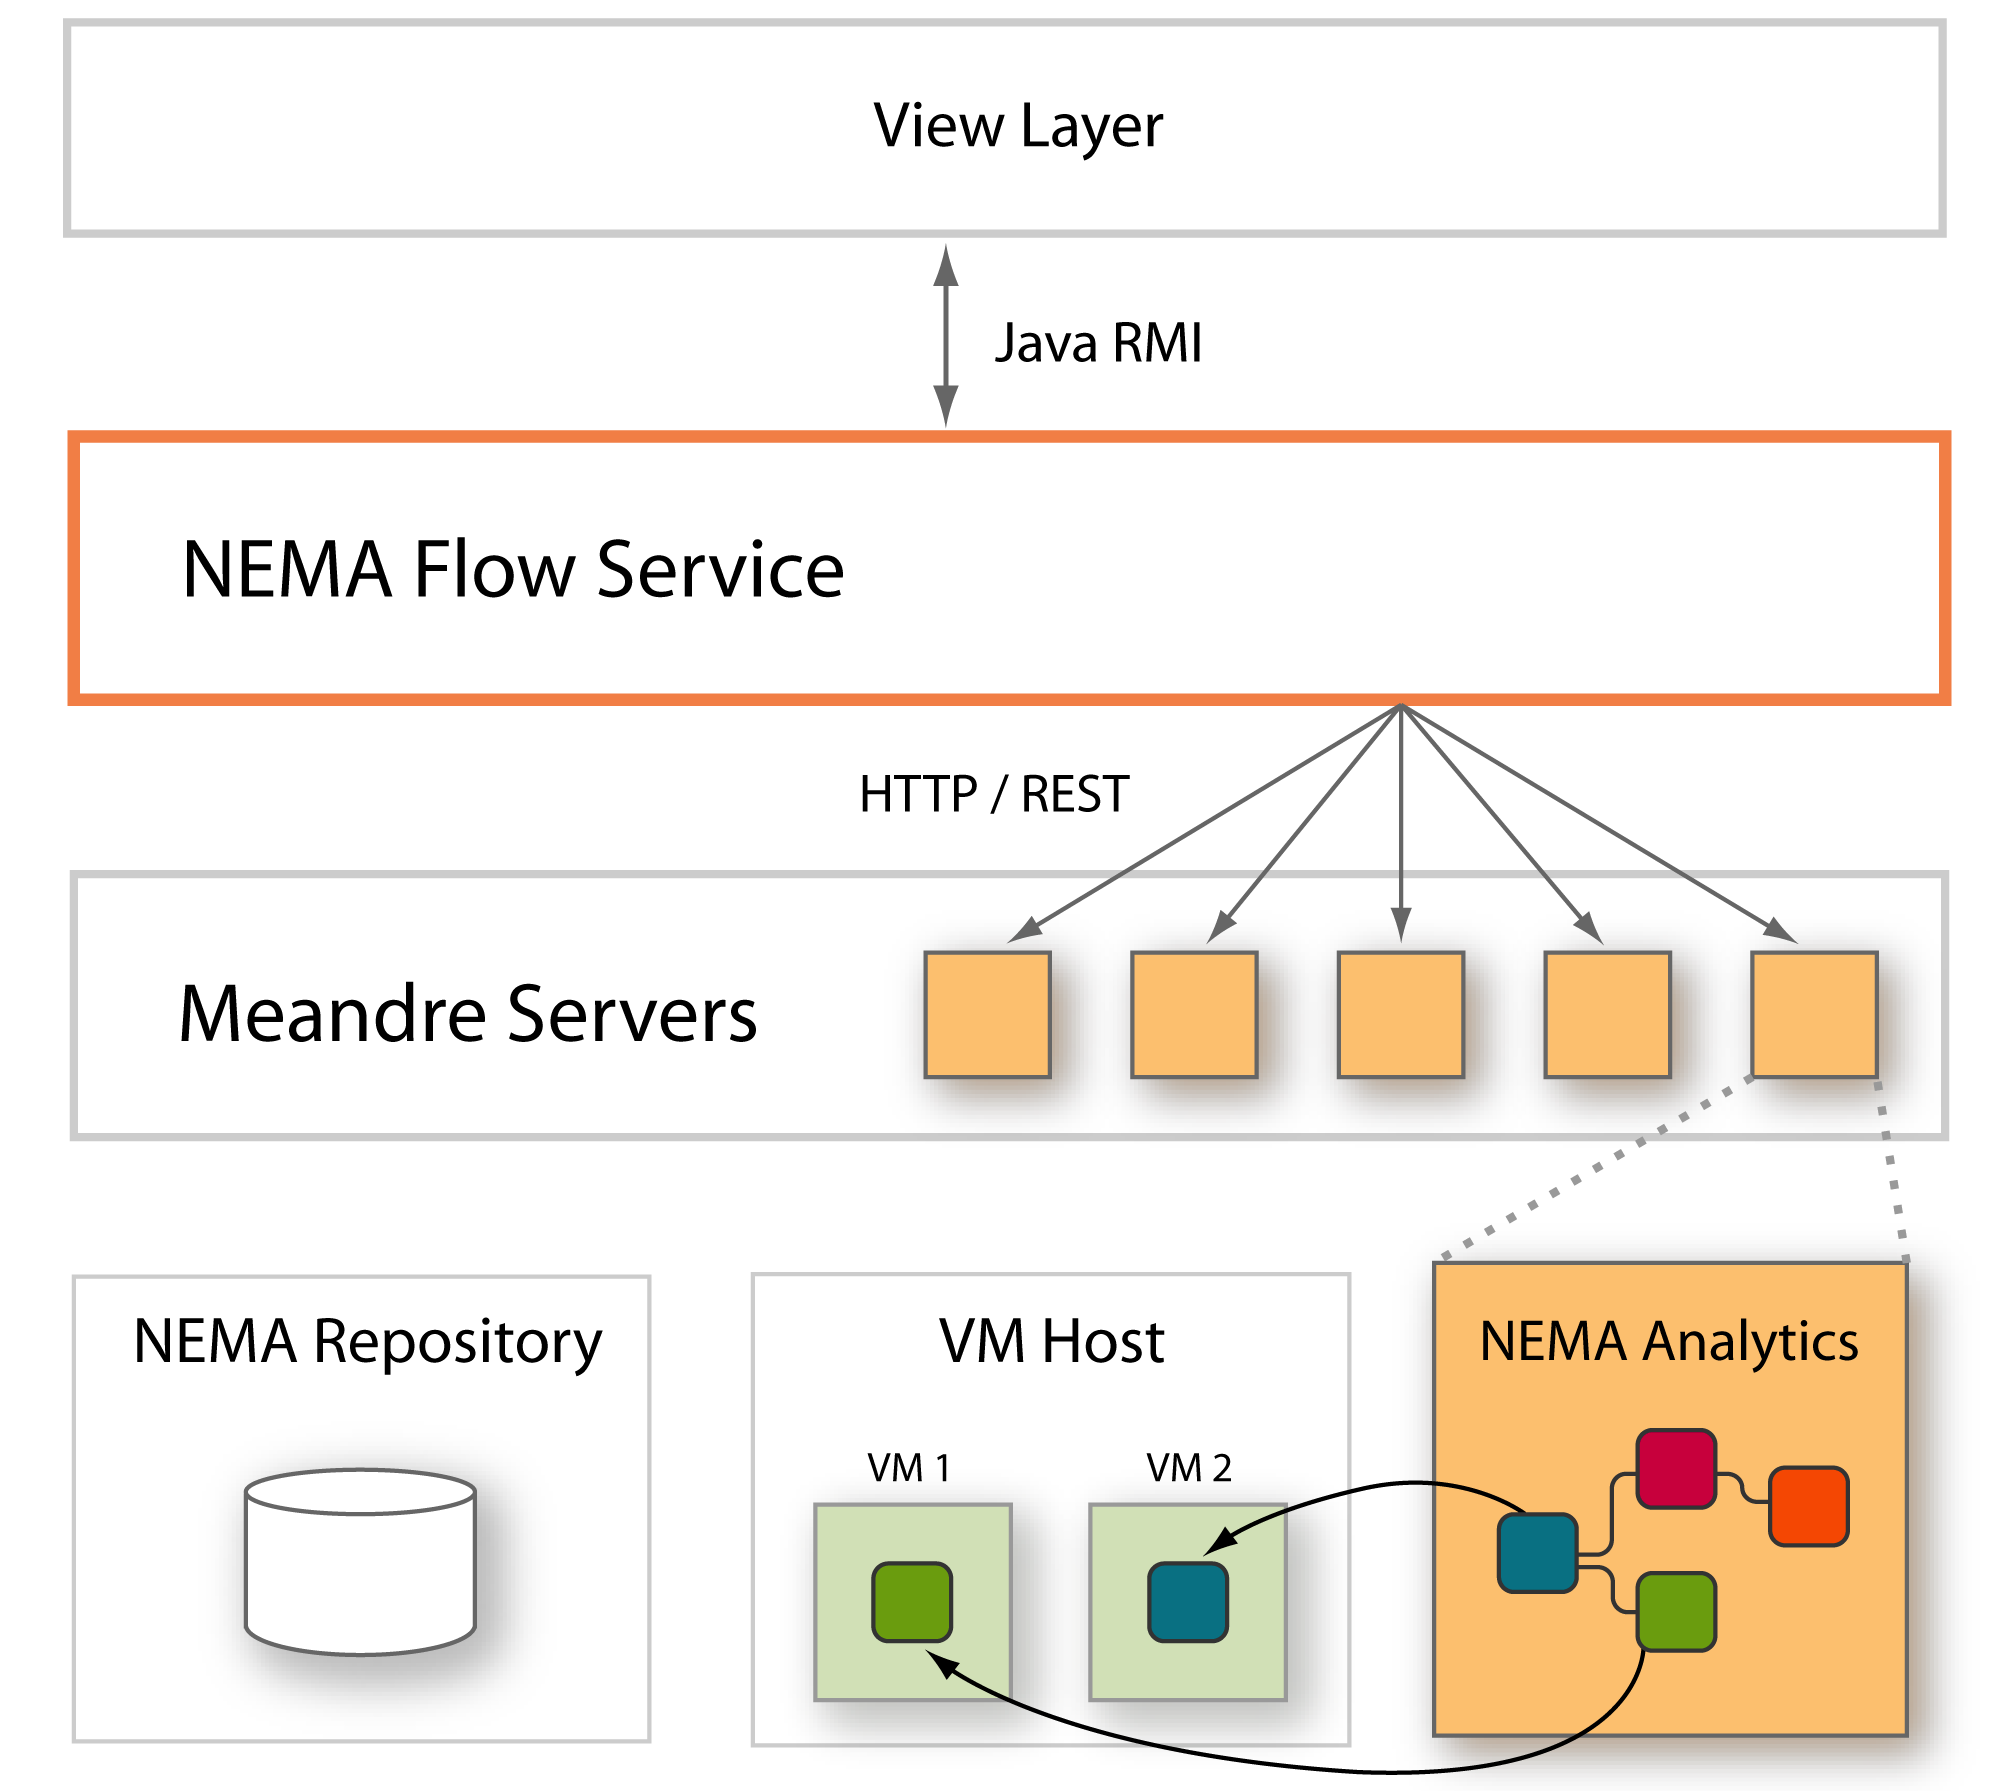
\includegraphics[width=2.8in]{infrastructure}
  \caption{An overview of the NEMA service infrastructure}
\label{fig_infrastructure}
\end{figure}
The NEMA infrastructure is initially intended to support component harnesses to execute Java, Matlab, VAMP API plugins \cite{cannam2006sonic} and arbitrary binary executables and shell scripts (that launch processes compatible with the host operating system and architecture). This provides an immediate path to integration of most, if not all software types and offers a model and examples for building more convenient hosts for particular languages or plugin environments. A diagrammatic overview of the NEMA service infrastructure and its workflow implementation in the Meandre framework is given in figure \ref{fig_infrastructure}.

% Workflow facilitates use of differing sites, dependencies and IO formats
By using a workflow approach to defining experiment tasks, those tasks are naturally broken down into discrete units or components which may be independently scheduled and distributed to satisfy collection access restrictions, software/architecture dependencies or IO file format requirements. For example a user of the NEMA service would be able to conduct an experiment in which:
\begin{enumerate}
\item a collection of tracks held at a remote site, which cannot be distributed, is analysed by Matlab code outputting into Weka's ARFF file format \cite{witten1999wpm}, 
\item the resulting audio analysis based features are raised into the data model and transmitted to another NEMA site with greater compute infrastructure, 
\item one or more machine learning frameworks or procedures are launched using automatically constructed shell commands, on specified Virtual Machine infrastructures, to predict a metadata field or transcription for each track, which is then serialized in a MIREX file format,
\item the MIREX format file is read and interpreted in the context of the experiment into the NEMA data model,
\item the results of the experiment are evaluated using Java-based MIR evaluation components provided by the NEMA project,
\item and finally both the prediction and evaluation data is exposed by the NEMA service in the standardised data model and eventually will be integrated into a linked data repository.
\end{enumerate}
%FIGURE experiment flow diagram showing differing sites, machine/VM hosts and IO formats  




\subsubsection{Experiment and Workflow Sharing}
%	Break up tasks into smaller units (multi-part feature extraction, classification, meta-classification)
The workflow sharing approach designed for NEMA has been modelled after the myExperiment Virtual Research Environment \cite{de2007designing} and directly addresses many of the same issues. It is expected that the NEMA service will fully integrate with myExperiment at some stage in the future.  This approach facilitates the easy sharing and reuse of experiment setups and partially or fully-specified implementations of those experiments. For example, a MIREX task may be defined in terms of a component to provide an input dataset and task description (e.g. classify music by genre), and number of required but unspecified process components (e.g. perform feature extraction, train classifier, apply classifier to test dataset) and an evaluation component. A participating lab would then configure components to perform each of the specified processes and execute the configured workflow to perform the task and receive evaluation results.  Similarly a researcher might publish an experiment definition (a fully defined task) and fully configured workflows or simply computed results representing experiments in published paper or thesis, allowing other researchers to accurately compare their work or build on the results.

%		drive cross-pollination - publication/sharing of working components
%				allows researchers to focus on their specific problem 
%					rather than having to re-implement standard procedures for comparison or reuse
%					lowers the bar to entry in to the field
%					(ref. myExperiment paper, issues section)
Further, if users choose to publish their components for re-use by other researchers, NEMA can drive the cross-pollination of research mitigating the need to re-implement techniques or learn additional languages/frameworks/applications. Further, this would lower the bar of entry in to particular areas of research, allow researchers to focus on their particular area rather than supporting technologies, provide recommendations and know-how on ways to address particular problems and will facilitate higher-level Musicological research in more reasonable time-scales, skill-sets and levels of effort than is presently possible.   
%				e.g. leverage chord transcription in score following or genere classification/tagging
%				combine onset detectors with F0 or multiple F0 estimators to produce full transcriptions
For example, a researcher might be able to leverage existing chord transcription systems in implementations of techniques for tasks such as score following, music description or search. Similarly, existing audio event-onset detection procedures might be combined with dominant F0 (melody) estimators and machine learning/IR frameworks to produce an index of melodies. 
%					Teaching tool?
Hence, the NEMA service may eventually form a ideal teaching tool for use in many fields including Musicology, Machine-learning, Library Information Science and MIR.

%	Automated evaluation/leaderboards
%		Automated result publication/dissemination
Finally, the provision of automated and standardised evaluation tools and result collections should facilitate (as MIREX has done in the past) better analysis, reporting and dissemination of results in the field of MIR than would otherwise be possible.
%		Based on new standardised, high-quality evaluation toolkit developed as part of project
The evaluation tools and IO/Interoperability framework developed to implement the NEMA service is also made available as an open-source toolkit for MIR experimentation and software building and, it is hoped, will be a significant resource to the community in of itself\footnote{source code and documentation for the NEMA project infrastructure is available from google code: \url{http://code.google.com/p/nemadiy}}. 
%immediately provides connects between AudioDB, jMIR, SOnic annotator and the Vamp API and the ACE/Weka machine learning frameworks
Out of the box, the toolkit will enable the interoperability of AudioDB \cite{casey2008audiodb}, jMIR \cite{mckay2009jmir}, Sonic Annotator and the VAMP API \cite{cannam2006sonic}, ACE \cite{mckay2005ace} and the Weka Machine-Learning toolkit \cite{witten1999wpm}.  


\subsubsection{Resource Resolution, Security and Attribution}
%security
Given that security is a prime concern for any NEMA-hosted collections, it is vital that the analysis code is sent to the data and that result data is only returned in a controlled model in which the transmission of the original audio content (or a reconstructable form thereof) may be prevented.
%	OMEN - extract feats at remote sites running infrastructure
The model for the extraction of MIR information on remote collections used in NEMA, which protects the NEMA-hosted music collections, is based on the On-demand Metadata Extraction Network (OMEN) \cite{mcennis2006overview} developed at the Schulich School of Music, McGill University.

% Resource resolution (varied encodings/sources)
% Access to resources
Format dependencies may also mean that multiple different encodings of the content may need to be maintained or conversion facilities provided. The ability to represent multiple sources for the content also facilitates better access to the resource as, for example, NEMA might not be able to provide streaming access to the controlled content for auditioning but could refer to a publicly or commercially accessible version of the content. \\

% security for data/code and publication/attribution
The security of code submitted to the NEMA service is also prime concern, as these components may or may not be under IP restriction or may not be ready for wide-spread distribution. Hence, the NEMA service allows users contributing component code to control the level of access of other users to their components (implementing a `some rights reserved' sharing model that may help promote academic work and experimentation that would otherwise be difficult or impossible), limited only by the fact that NEMA will never permit the download of component code to non-NEMA managed servers.
  %	Collection of author data/attribution/citation data?
Additionally, full author attribution information and citation information is captured with each component profile in order to facilitate correct attribution in cases of reuse and the viewing of the components themselves as collections of documents and metadata. 
%		Treat code and its metadata as data?

\subsection{Using and re-using the NEMA service}
%	Users can try to solve their own problems
The existing approach to the running of MIREX evaluations involves the hand execution of extremely diverse pieces of code by around a half dozen research students over short period of time and may therefore be considered expensive in terms of human resources.  One of the key advantages of the NEMA `self-service' infrastructure is that it exposes, in a controlled manner, the configuration of component execution to the user. This enables the user to solve their own issues, in such a way that, they can rapidly make corrections/alterations to their own codebase or configuration to produce a successful run, avoiding the often drawn out testing, email communication, bug report and update cycles that incurred each year at MIREX.
 
%	MIREX - Testing datasets (can't even share those at times!)
Further, this issue is often exacerbated by the difficulty of providing test datasets for tasks, as even these are often impossible to share due to copyright issues or the impact it would have on already limited dataset sizes. However, NEMA is of course able to provide test datasets within the NEMA service to facilitate rapid testing of component code before long runs are executed. 

%	Potential for VM use to support other architectures/languages/dependencies
Finally, the NEMA service embraces a Virtual Machine Infrastructure for the execution of component code, where necessary. Throughout the hosting of five years of MIREX evaluations the IMIRSEL team has encountered a wide variety of dependency requirements and has developed/maintains a linux based compute cluster node image satisfying as many of these dependencies as possible within a single image. However, there are always special cases, particularly including platform dependencies on Windows operating systems and non-standard libraries. Hence, a range of VM images will be maintained for use by third party components.
%		VM customisation??
Eventually, it is hoped, a user customisable VM container system will be exposed (allowing a user to login to an existing image, modify it for their use in a limited fashion and save it for later reuse).
%		Sandboxing
Obviously, such modified VMs or indeed any VM running potentially unknown code must be suitably sand-boxed and will be permitted: read access only to its component code and data required for a particular experiment or task; write access only to specified scratch and output locations; will be required to return its output in certain specified formats, such that it may be appropriately inspected or interpreted; and no access to the outside world.

\subsubsection{Exposing Results, Metadata, Predictions and Provenance}
%unique ids, persistent storage
The NEMA service infrastructure provides each task execution with a unique identifier and persistent storage of logs, execution information / provenance, predictions and evaluation results. This data may be published by a user within NEMA so that it maybe accessed by the community through either a provided digital library framework (Greenstone \cite{witten2000greenstone}) or linked data repository/SPARQL endpoint. 
%Predict/extract data that is not available\\
The design of the linked data system or \emph{repository} for the NEMA project is beyond the scope of this paper. However, it is hoped that the NEMA service infrastructure will one day be used to provide on-demand processing required to satisfy queries submitted via the repository endpoint (i.e. extracting and/or predicting metadata for content that is not already known).

\section{Implementation}
NEMA uses Meandre\footnote{\url{http://seasr.org/meandre/}} to implement its worklow processes. Meandre is a semantic-web-driven data-intensive flow execution environment. Meandre provides basic infrastructure for data-intensive computation. It provides a high-level language to describe flows and both a multicore and distributed execution environment based on a service-oriented paradigm. The Meandre Infrastructure provides a plugin model similar to the servlets in a Java Enterprise Enviornment where  custom functionality can be implemented, NEMA uses plugins to make data sources available as a JNDI \cite{lee2000jndi} resource to all the tasks.
%
%The Meandre Infrastructure allows NEMA to Monitor the lifecycle of a task.  The task is submitted to the NEMA Flow Service, that schedules the experiment to run on one of the Meandre Servers. The Meandre Servers assembles the experiment by downloading the work flow definitions and code from possibly distributed locations and starts the execution. 
%
%The flow execution can depend upon a Virtual machine with a preset execution environment, such as a particular version of python, JVM or other libraries The NEMA Executor Service runs on each virtual machine and handles the process execution and the lifecycle of the process. It  reports back to the flow asynchronously the success or failure of the process. The artifacts produced by the process are serialized and moved to the flow server as input to the next the component. We are currently working on an implementation that would store the results in a central NEMA Repository service based on  Flexible and Extensible Digital Object and Repository Architecture (Fedora) \cite{payette-flexible} with a client interface that would allow tasks to retrieve the artifacts.
%
% conference papers do not normally have an appendix

% use section* for acknowledgement
\section*{Acknowledgment}
The NEMA project is funded by the Andrew W. Mellon foundation. The authors would also like to acknowledge the contributions of the NEMA project team at the IMIRSEL laboratory at UIUC and the project partners from the Universities of McGill, Southampton, Waikato, Goldsmiths University of London and Queen Mary's University of London.




% trigger a \newpage just before the given reference
% number - used to balance the columns on the last page
% adjust value as needed - may need to be readjusted if
% the document is modified later
%\IEEEtriggeratref{8}
% The "triggered" command can be changed if desired:
%\IEEEtriggercmd{\enlargethispage{-5in}}

% references section

% can use a bibliography generated by BibTeX as a .bbl file
% BibTeX documentation can be easily obtained at:
% http://www.ctan.org/tex-archive/biblio/bibtex/contrib/doc/
% The IEEEtran BibTeX style support page is at:
% http://www.michaelshell.org/tex/ieeetran/bibtex/
%\bibliographystyle{IEEEtran}
% argument is your BibTeX string definitions and bibliography database(s)
%\bibliography{IEEEabrv,../bib/paper}
%
% <OR> manually copy in the resultant .bbl file
% set second argument of \begin to the number of references
% (used to reserve space for the reference number labels box)

\bibliographystyle{IEEEtran} 
\bibliography{IEEEabrv,references}




% that's all folks
\end{document}


